\documentclass{beamer}
\usepackage[utf8]{inputenc}

\usetheme{Madrid}
\usecolortheme{default}
\usepackage{amsmath,amssymb,amsfonts,amsthm}
\usepackage{txfonts}
\usepackage{tkz-euclide}
\usepackage{listings}
\usepackage{adjustbox}
\usepackage{array}
\usepackage{tabularx}
\usepackage{gvv}
\usepackage{lmodern}
\usepackage{circuitikz}
\usepackage{tikz}
\usepackage{graphicx}

\setbeamertemplate{page number in head/foot}[totalframenumber]

\usepackage{tcolorbox}
\tcbuselibrary{minted,breakable,xparse,skins}



\definecolor{bg}{gray}{0.95}
\DeclareTCBListing{mintedbox}{O{}m!O{}}{%
  breakable=true,
  listing engine=minted,
  listing only,
  minted language=#2,
  minted style=default,
  minted options={%
    linenos,
    gobble=0,
    breaklines=true,
    breakafter=,,
    fontsize=\small,
    numbersep=8pt,
    #1},
  boxsep=0pt,
  left skip=0pt,
  right skip=0pt,
  left=25pt,
  right=0pt,
  top=3pt,
  bottom=3pt,
  arc=5pt,
  leftrule=0pt,
  rightrule=0pt,
  bottomrule=2pt,
  toprule=2pt,
  colback=bg,
  colframe=orange!70,
  enhanced,
  overlay={%
    \begin{tcbclipinterior}
    \fill[orange!20!white] (frame.south west) rectangle ([xshift=20pt]frame.north west);
    \end{tcbclipinterior}},
  #3,
}
\lstset{
    language=C,
    basicstyle=\ttfamily\small,
    keywordstyle=\color{blue},
    stringstyle=\color{orange},
    commentstyle=\color{green!60!black},
    numbers=left,
    numberstyle=\tiny\color{gray},
    breaklines=true,
    showstringspaces=false,
}
%------------------------------------------------------------
%This block of code defines the information to appear in the
%Title page
\title %optional
{3.2.29}
%\subtitle{A short story}

\author % (optional)
{Gautham-AI25BTECH11013}



\begin{document}


\frame{\titlepage}
\begin{frame}{Question}
Construct a $\triangle ABC$ given 
\begin{align}
a = BC = 6\ \text{cm},\qquad \angle B = 30^\circ,\qquad AC - AB = 4\ \text{cm}.\\
\end{align}
\end{frame}

\begin{frame}{Theoretical Solution}
In the usual notation $a=BC,\; b=CA,\; c=AB$.  From the cosine formula in $\triangle ABC$\\
\begin{align}
b^2 = a^2 + c^2 - 2ac\cos B. 
\end{align}
Put $b = c + k$ where $k = 4$. 
\begin{align}
(c+k)^2 = a^2 + c^2 - 2ac\cos B.
\end{align}
Canceling $c^2$ and collecting terms in $c$:
\begin{align}
2kc + k^2 = a^2 - 2ac\cos B
\quad\Longrightarrow\quad
c\big(2k + 2a\cos B\big) = a^2 - k^2.
\end{align}
       Hence the general expression for $c$ when $b-c=k$ is
\begin{align}
\boxed{ c =\frac{a^2 - k^2}{2(k + a\cos B)} }. 
\end{align} 
\end{frame}
\begin{frame}{Theoretical solution}

Now substitute $a=6,\; B=30^\circ,\; k=4$:
\begin{align}
\cos 30^\circ = \frac{\sqrt3}{2},\qquad
c = \frac{6^2 - 4^2}{2\big(4 + 6\cos 30^\circ\big)}
= \frac{36 - 16}{2\big(4 + 6\cdot\frac{\sqrt3}{2}\big)}
= \frac{20}{2\big(4 + 3\sqrt3\big)}.
\end{align}
Numerically,
\begin{align}
c \approx 1.09\ \text{cm},\qquad b = c + 4 \approx 5.09\ \text{cm}.
\end{align}
Place $\Vec{B}=\myvec{0 \\ 0}$ and $\Vec{C}=\myvec{a \\ 0}=\myvec{6 \\ 0}$.
Point $A$ lies on this ray with $BA=c$, so
\begin{align}
\Vec{A}=c\myvec{\cos B \\ \sin B}
\approx (0.94, 0.54).
\end{align}
\end{frame}
\begin{frame}[fragile]
\frametitle{Python Code}
   \begin{lstlisting}
 import sys                                     
sys.path.insert(0, '/home/gauthamp/Documents/codes/CoordGeo')  
import numpy as np
import numpy.linalg as LA
import matplotlib.pyplot as plt
import matplotlib.image as mpimg

#local imports
from line.funcs import *
from triangle.funcs import *
from conics.funcs import circ_gen
theta = 30
#Given points
B = np.array(([0, 0])).reshape(-1,1) 
C = np.array(([6, 0])).reshape(-1,1)  
A= 1.09*np.array(([np.cos(np.deg2rad(theta)),np.sin(np.deg2rad(theta))])).reshape(-1,1)  
   \end{lstlisting}
\end{frame}
\begin{frame}[fragile]
\frametitle{Python Code}
   \begin{lstlisting}
#Generating all lines
x_AB = line_gen(A,B)
x_BC = line_gen(B,C)
x_CA = line_gen(C,A)
plt.plot(x_AB[0,:],x_AB[1,:],label='$AB$')
plt.plot(x_BC[0,:],x_BC[1,:],label='$BC$')
plt.plot(x_CA[0,:],x_CA[1,:],label='$CA$')
colors = np.arange(1,4)
tri_coords = np.block([[A,B,C]])
plt.scatter(tri_coords[0,:], tri_coords[1,:], c=colors)
vert_labels = ['A','B','C']
for i, txt in enumerate(vert_labels):
    #plt.annotate(txt, # this is the text
    plt.annotate(f'{txt}\n({tri_coords[0,i]:.2f}, {tri_coords[1,i]:.2f})',
                 (tri_coords[0,i], tri_coords[1,i]), textcoords="offset points", xytext=(25,5), ha='center') 
 \end{lstlisting}
\end{frame}
\begin{frame}[fragile]
\frametitle{Python Code}
   \begin{lstlisting}
ax = plt.gca()
ax.spines['top'].set_color('none')
ax.spines['left'].set_position('zero')
ax.spines['right'].set_color('none')
ax.spines['bottom'].set_position('zero')
'''
ax.spines['left'].set_visible(False)
ax.spines['right'].set_visible(False)
ax.spines['top'].set_visible(False)
ax.spines['bottom'].set_visible(False)
plt.xlabel('$x$')
plt.ylabel('$y$')
plt.legend(loc='best')
plt.grid() 
plt.axis('equal')
plt.savefig('/home/gauthamp/ee1030-2025/ai25btech11013/matgeo/3.2.29/figs/fig.png')
plt.show() 
   \end{lstlisting}
\end{frame}
\begin{frame}{Figure}
    \begin{figure}[h!]
    \centering
    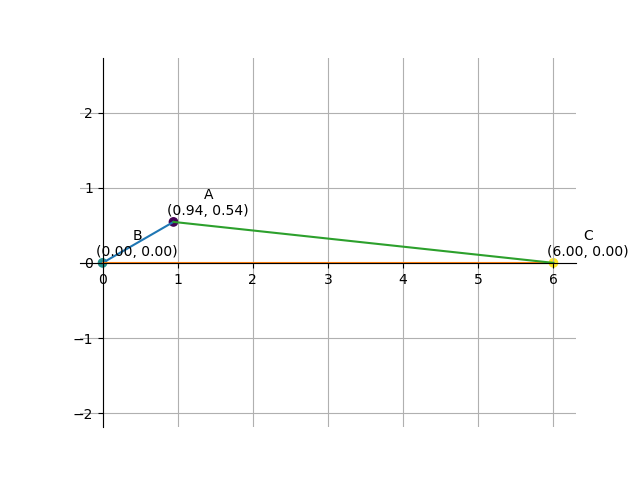
\includegraphics[height=0.6\textheight, keepaspectratio]{figs/fig.png}
    \label{figure_1}
\end{figure}
\end{frame}
\end{document}
